\documentclass[a4paper]{article}

\usepackage{fullpage}

\usepackage{graphicx}
\usepackage{caption}
\usepackage{subcaption}

\usepackage{amsmath}

% Code for typesttting C code
\usepackage{listings}
\usepackage{color}

\definecolor{mygreen}{rgb}{0,0.6,0}
\definecolor{mygray}{rgb}{0.5,0.5,0.5}
\definecolor{mymauve}{rgb}{0.58,0,0.82}
\definecolor{mybrown}{rgb}{0.5,0,0}

\lstdefinestyle{MyCStyle}{ %
  language=C,                      % the language of the code
  backgroundcolor=\color{white},   % choose the background color; you must add \usepackage{color} or \usepackage{xcolor}
  basicstyle=\ttfamily    ,        % the size of the fonts that are used for the code
  breakatwhitespace=false,         % sets if automatic breaks should only happen at whitespace
  breaklines=true,                 % sets automatic line breaking
  captionpos=b,                    % sets the caption-position to bottom
  commentstyle=\color{mygreen},    % comment style
  deletekeywords={...},            % if you want to delete keywords from the given language
  escapeinside={\%*}{*)},          % if you want to add LaTeX within your code
  extendedchars=true,              % lets you use non-ASCII characters; for 8-bits encodings only, does not work with UTF-8
  frame=single,                    % adds a frame around the code
  keepspaces=true,                 % keeps spaces in text, useful for keeping indentation of code (possibly needs columns=flexible)
  keywordstyle=\color{blue},       % keyword style
  morecomment=[l][\color{mybrown}]\#,  % compiler directive
  morekeywords={*,...},            % if you want to add more keywords to the set
  numbers=left,                    % where to put the line-numbers; possible values are (none, left, right)
  numbersep=5pt,                   % how far the line-numbers are from the code
  numberstyle=\tiny\color{mygray}, % the style that is used for the line-numbers
  rulecolor=\color{black},         % if not set, the frame-color may be changed on line-breaks within not-black text (e.g. comments (green here))
  showspaces=false,                % show spaces everywhere adding particular underscores; it overrides 'showstringspaces'
  showstringspaces=false,          % underline spaces within strings only
  showtabs=false,                  % show tabs within strings adding particular underscores
  stepnumber=1,                    % the step between two line-numbers. If it's 1, each line will be numbered
  stringstyle=\color{mymauve},     % string literal style
  tabsize=2,                       % sets default tabsize to 2 spaces
  title=\lstname                   % show the filename of files included with \lstinputlisting; also try caption instead of title
}

\lstdefinestyle{MyASMStyle}{ %
  language=[x86masm]Assembler,     % the language of the code
  backgroundcolor=\color{white},   % choose the background color; you must add \usepackage{color} or \usepackage{xcolor}
  basicstyle=\ttfamily    ,        % the size of the fonts that are used for the code
  breakatwhitespace=false,         % sets if automatic breaks should only happen at whitespace
  breaklines=true,                 % sets automatic line breaking
  captionpos=b,                    % sets the caption-position to bottom
  commentstyle=\color{mygreen},    % comment style
  deletekeywords={...},            % if you want to delete keywords from the given language
  escapeinside={\%*}{*)},          % if you want to add LaTeX within your code
  extendedchars=true,              % lets you use non-ASCII characters; for 8-bits encodings only, does not work with UTF-8
  frame=single,                    % adds a frame around the code
  keepspaces=true,                 % keeps spaces in text, useful for keeping indentation of code (possibly needs columns=flexible)
  keywordstyle=\color{blue},       % keyword style
  morecomment=[l][\color{mybrown}]\#,  % compiler directive
  morekeywords={*,...},            % if you want to add more keywords to the set
  numbers=left,                    % where to put the line-numbers; possible values are (none, left, right)
  numbersep=5pt,                   % how far the line-numbers are from the code
  numberstyle=\tiny\color{mygray}, % the style that is used for the line-numbers
  rulecolor=\color{black},         % if not set, the frame-color may be changed on line-breaks within not-black text (e.g. comments (green here))
  showspaces=false,                % show spaces everywhere adding particular underscores; it overrides 'showstringspaces'
  showstringspaces=false,          % underline spaces within strings only
  showtabs=false,                  % show tabs within strings adding particular underscores
  stepnumber=1,                    % the step between two line-numbers. If it's 1, each line will be numbered
  stringstyle=\color{mymauve},     % string literal style
  tabsize=2,                       % sets default tabsize to 2 spaces
  title=\lstname                   % show the filename of files included with \lstinputlisting; also try caption instead of title
}

\newlength{\pic}

\begin{document}

\title{EE445M Lab 4 Report}
\author{Yen-Kai Huang \\ Siavash Zanganeh Kamali}
\maketitle

\section{Objective} The goal of this lab is to learn the DSP theory of building a digital FIR filter. We also
familiarize ourselves with theories behind and tools for building an analog filter. We will make use of the OS
from Lab 3 and write a oscilloscope-spectrum analyser application with a LCD display.

\section{Hardware Design} 

\setlength{\pic}{0.75\textwidth}
\begin{figure}[htp]
	\center
	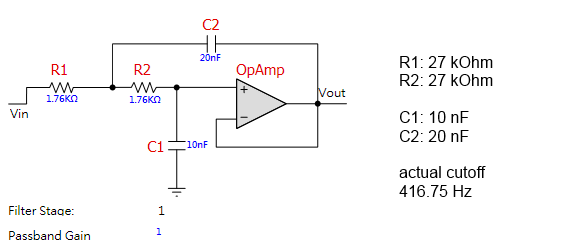
\includegraphics[width=\pic]{filterdesign}
\end{figure}

\section{Software Design}
Below is the code for sampling and acquiring the data.

\lstset{language=C, style=MyCStyle}
\lstinputlisting{Code/consumer.c}

It uses the following filter code on input if specified to do so.

\lstset{language=C, style=MyCStyle}
\lstinputlisting{Code/fir.c}

The result will be displayed on the LCD with the following thread.

\lstset{language=C, style=MyCStyle}
\lstinputlisting{Code/display.c}

The details setting of display mode, triggering mode of FFT (Once, Button-triggered, Continuous) and
the use of the FIR filter can all be adjusted in real time with the following Interpreter commands.

\lstset{language=C, style=MyCStyle}
\lstinputlisting{Code/interpreter_cmds.c}


\section{Measurement}
\paragraph{(a) Dynamic circuit performance (procedure 2)}

\begin{center}
\begin{tabular}{|l|l|l|l|}
\hline
\multicolumn{4}{|c|}{Analog Filter Performance Measurement} \\
\hline
freq & input voltage & output voltage & gain \\
\hline
100 & 1.58 & 1.58 & 1 \\
200 & 1.58 & 1.52 & 0.962025316 \\
300 & 1.58 & 1.36 & 0.860759494 \\
400 & 1.58 & 1.14 & 0.721518987 \\
500 & 1.58 & 0.9 & 0.569620253 \\
700 & 1.58 & 0.6 & 0.379746835 \\
1000 & 1.58 & 0.38 & 0.240506329 \\
1500 & 1.58 & 0.22 & 0.139240506 \\
2000 & 1.58 & 0.18 & 0.113924051 \\
\hline
\end{tabular}
\label{Analog}\\[5pt]
\textbf{Table 1.\ Analog Filter Performance Measurement}
\end{center}

\setlength{\pic}{0.8\textwidth}
\begin{figure}[htp]
\center
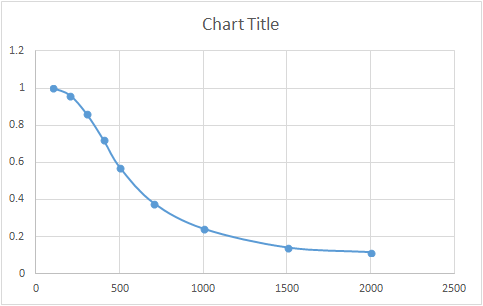
\includegraphics[width=\pic]{Plots/Procedure2}
\caption{Plot of analog filter performance measurement}
\end{figure}


\paragraph{(b) Digital scope data for each of the three frequencies (three by three = 9 graphs) (procedure 3) \\}
The result is shown Figure\,\ref{fig:Procedure3}. The pictures of LCD screens have been edited for better clarity.

\newlength{\pica}
\newlength{\picb}
\newlength{\picc}


\setlength{\pica}{0.28\textwidth}
\setlength{\picb}{0.4\textwidth}
\setlength{\picc}{0.4\textwidth}

\begin{figure}[htp]
\center
	\begin{subfigure}[H]{\pica}
	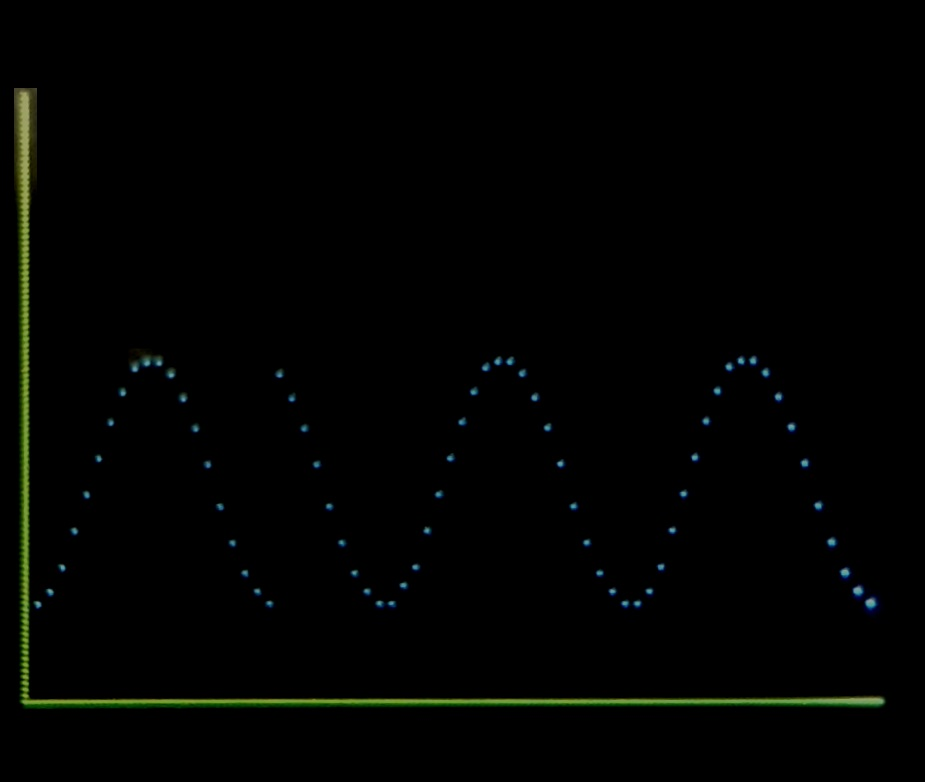
\includegraphics[width=\pica]{Images/100Hz}
	\caption{Digital scope data frequency = 100 Hz}
	\end{subfigure}
	\hfill
	\begin{subfigure}[H]{\pica}
	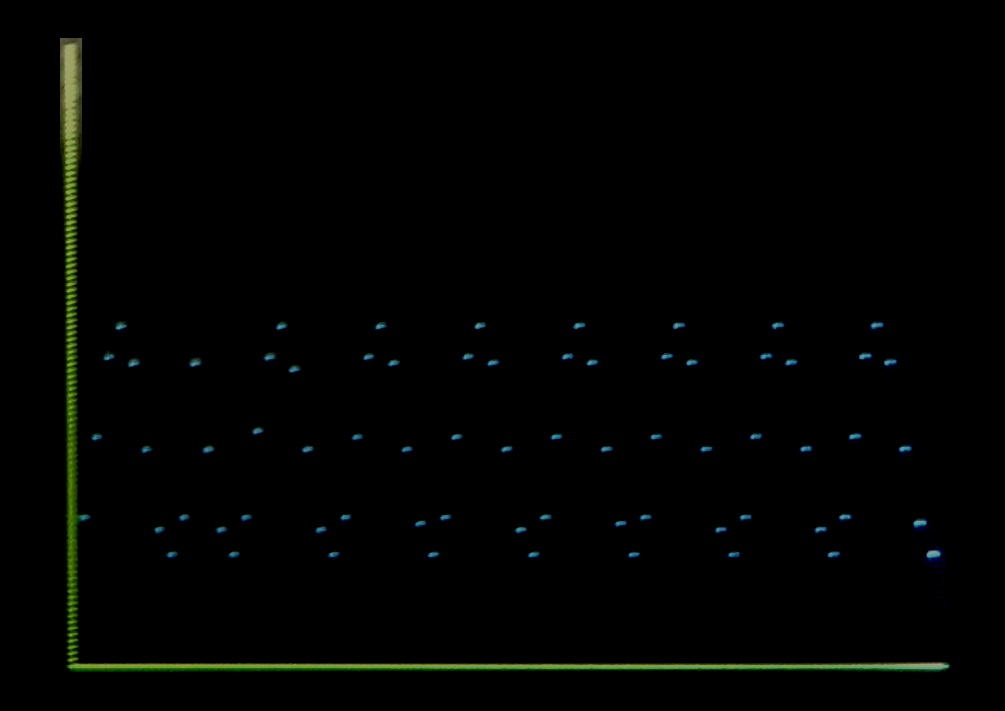
\includegraphics[width=\pica]{Images/250Hz}
	\caption{Digital scope data frequency = 250 Hz}
	\end{subfigure}
	\hfill
	\begin{subfigure}[H]{\pica}
	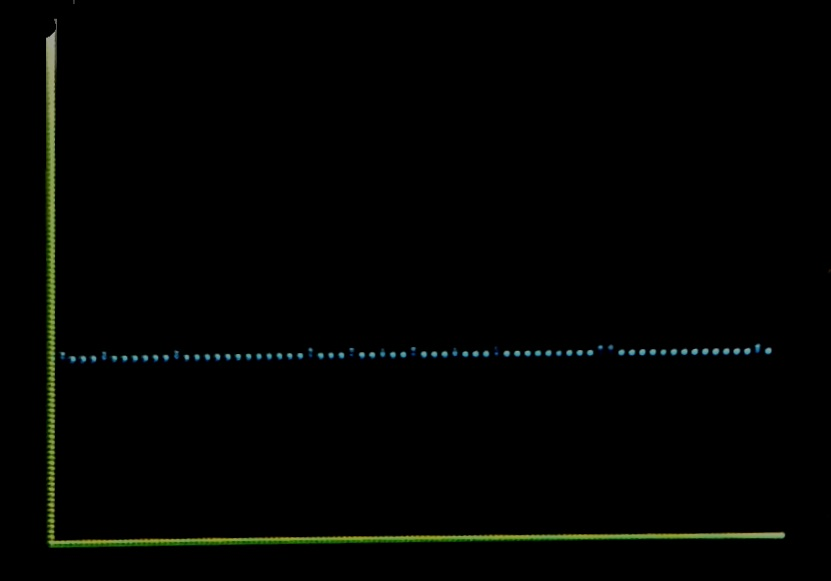
\includegraphics[width=\pica]{Images/2kHz}
	\caption{Digital scope data frequency = 2 kHz}
	\end{subfigure}	
	\\
	\begin{subfigure}[H]{\picb}
	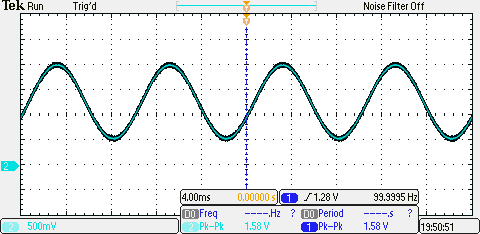
\includegraphics[width=\picb]{oscilloscope/fir100}
	\caption{Spectrum analyzer data}
	\end{subfigure}
	\begin{subfigure}[H]{\picc}
	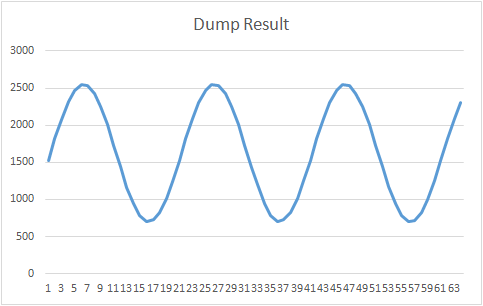
\includegraphics[width=\picc]{Plots/P3_100}
	\caption{print data}
	\end{subfigure}
	\\
	\begin{subfigure}[H]{\picb}
	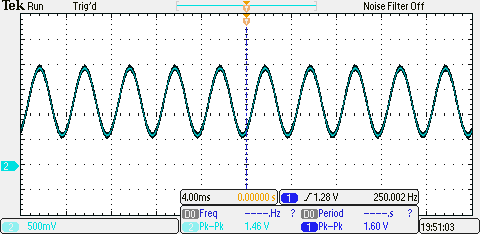
\includegraphics[width=\picb]{oscilloscope/fir250}
	\caption{Spectrum analyzer data}
	\end{subfigure}
	\begin{subfigure}[H]{\picc}
	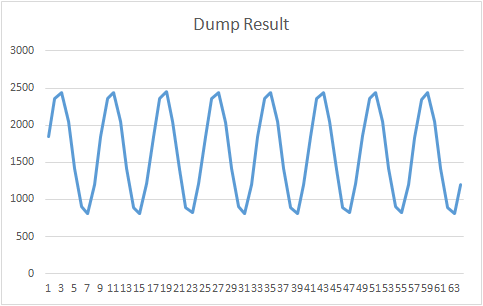
\includegraphics[width=\picc]{Plots/P3_250}
	\caption{print data}
	\end{subfigure}
	\\
	\begin{subfigure}[H]{\picb}
	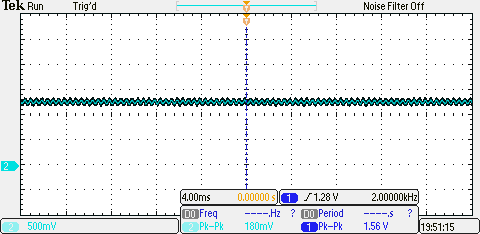
\includegraphics[width=\picb]{oscilloscope/fir2000}
	\caption{Spectrum analyzer data}
	\end{subfigure}
	\begin{subfigure}[H]{\picc}
	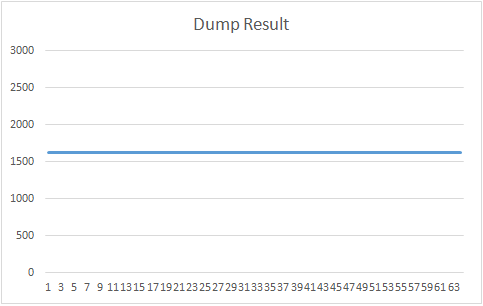
\includegraphics[width=\picc]{Plots/P3_2000}
	\caption{print data}
	\end{subfigure}
\caption{Plots and scope pictures}
\label{fig:Procedure3}
\end{figure}

\paragraph{(c) Spectrum analyzer data (three by three = 9 graphs) (procedure 3) \\}
See Figure\,\ref{fig:Procedure3FFT}

\setlength{\pica}{0.28\textwidth}
\setlength{\picb}{0.4\textwidth}
\setlength{\picc}{0.4\textwidth}

\begin{figure}[htp]
\center
	\begin{subfigure}[H]{\pica}
	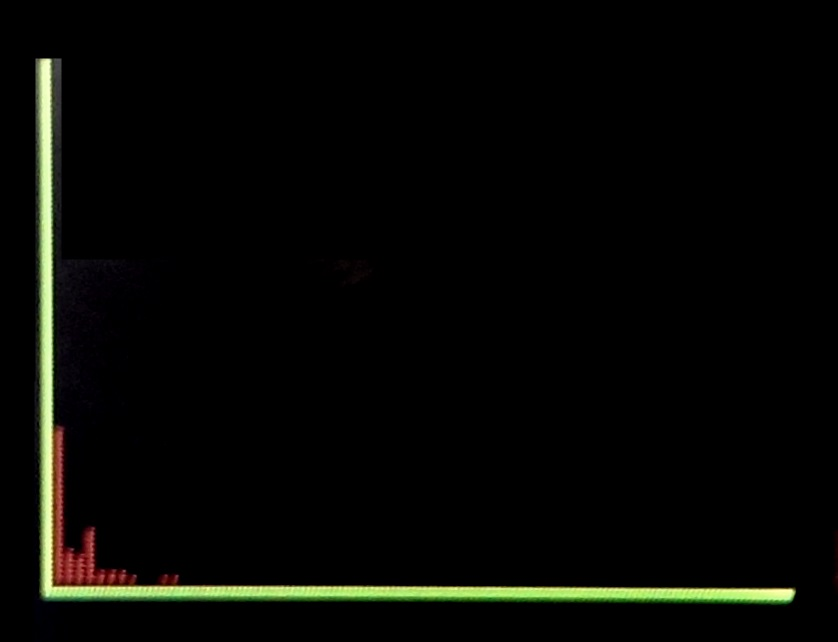
\includegraphics[width=\pica]{Images/FFT100}
	\caption{Digital scope data frequency = 100 Hz}
	\end{subfigure}
	\hfill
	\begin{subfigure}[H]{\pica}
	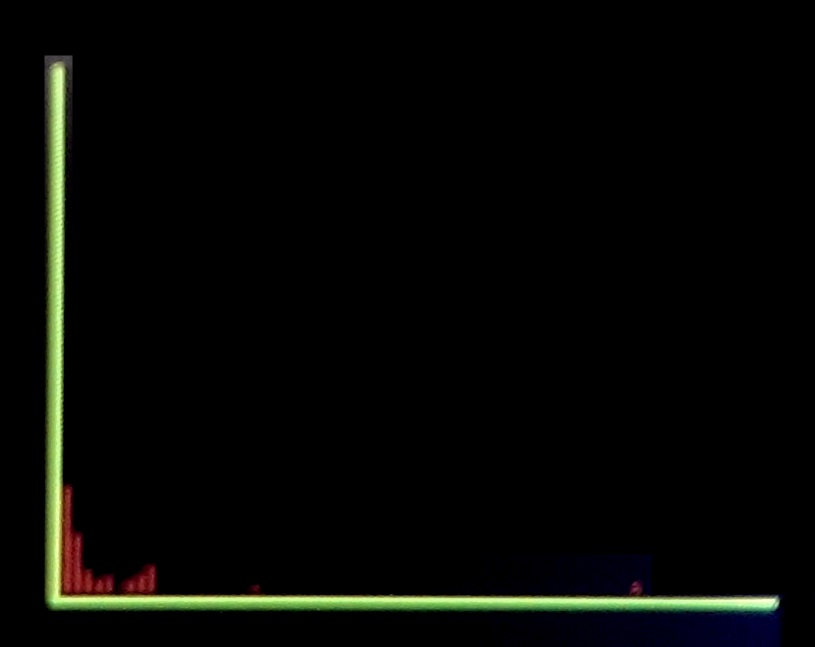
\includegraphics[width=\pica]{Images/FFT250}
	\caption{Digital scope data frequency = 250 Hz}
	\end{subfigure}
	\hfill
	\begin{subfigure}[H]{\pica}
	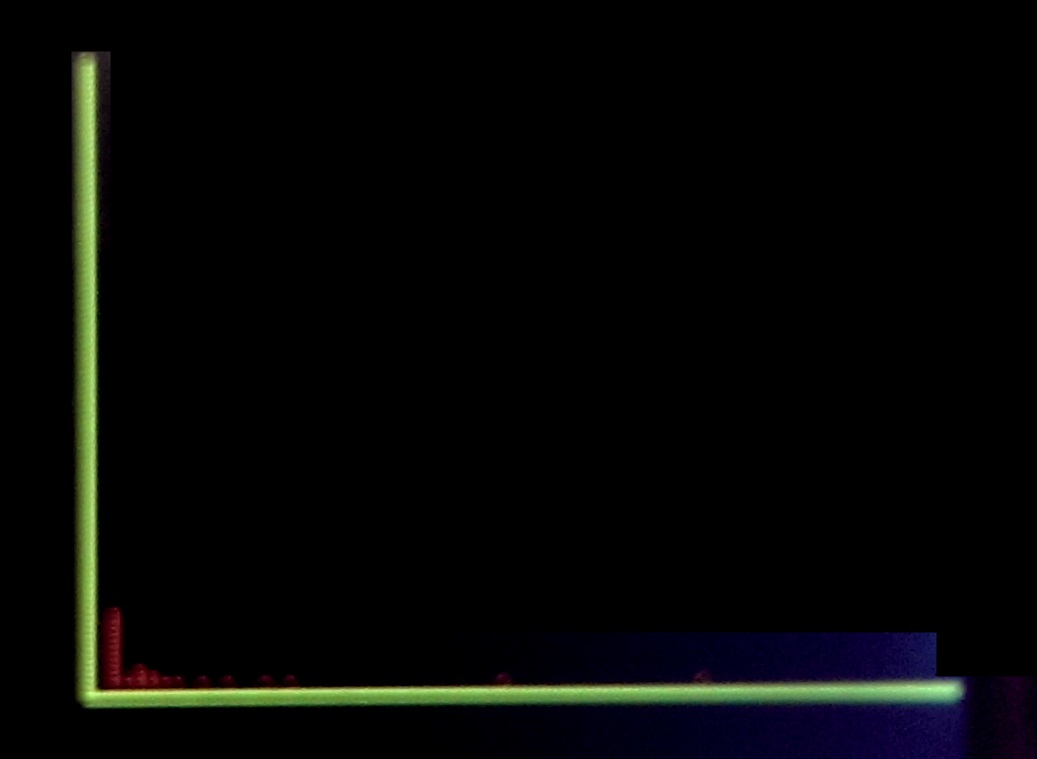
\includegraphics[width=\pica]{Images/FFT2000}
	\caption{Digital scope data frequency = 2 kHz}
	\end{subfigure}	
	\\
	\begin{subfigure}[H]{\picb}
	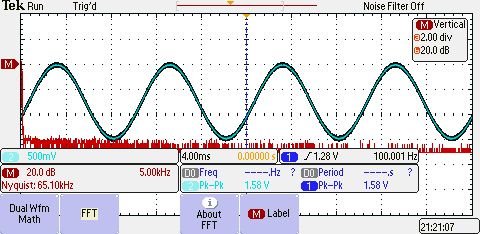
\includegraphics[width=\picb]{oscilloscope/fft100}
	\caption{Spectrum analyzer data}
	\end{subfigure}
	\begin{subfigure}[H]{\picc}
	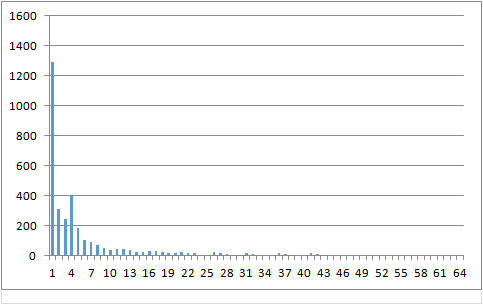
\includegraphics[width=\picc]{Plots/P3_FFT100}
	\caption{print data}
	\end{subfigure}
	\\
	\begin{subfigure}[H]{\picb}
	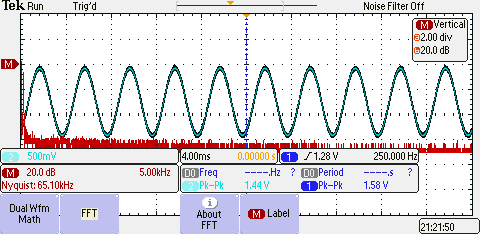
\includegraphics[width=\picb]{oscilloscope/fft250}
	\caption{Spectrum analyzer data}
	\end{subfigure}
	\begin{subfigure}[H]{\picc}
	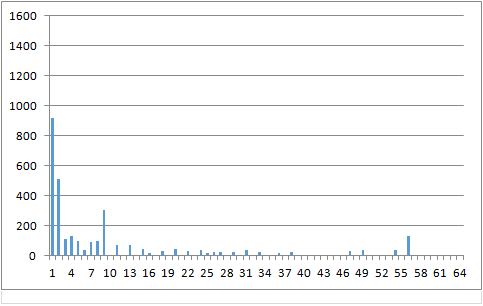
\includegraphics[width=\picc]{Plots/P3_FFT250}
	\caption{print data}
	\end{subfigure}
	\\
	\begin{subfigure}[H]{\picb}
	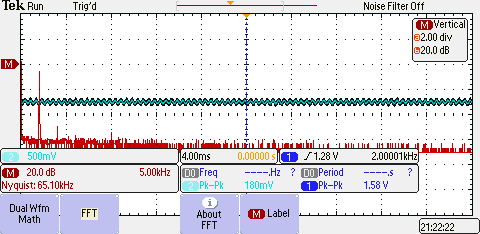
\includegraphics[width=\picb]{oscilloscope/fft2000}
	\caption{Spectrum analyzer data}
	\end{subfigure}
	\begin{subfigure}[H]{\picc}
	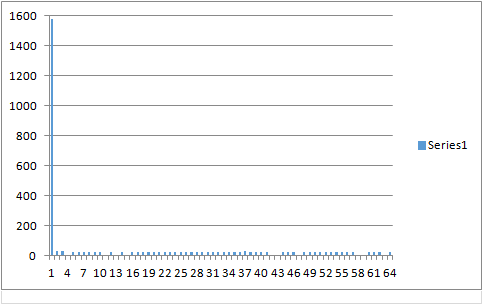
\includegraphics[width=\picc]{Plots/P3_FFT2000}
	\caption{print data}
	\end{subfigure}
\caption{Plots and scope pictures}
\label{fig:Procedure3FFT}
\end{figure}

\paragraph{(d) FIR filter test data (procedure 4) \\}
We imitated the turning of a robot by moving the sensor close to a wall surface and then move away.
The data collected is shown.

See Figure\,\ref{fig:Procedure4}

\setlength{\pica}{4cm}
\setlength{\picb}{8cm}

\begin{figure}[htp]
\center
\begin{subfigure}[H]{\pica}
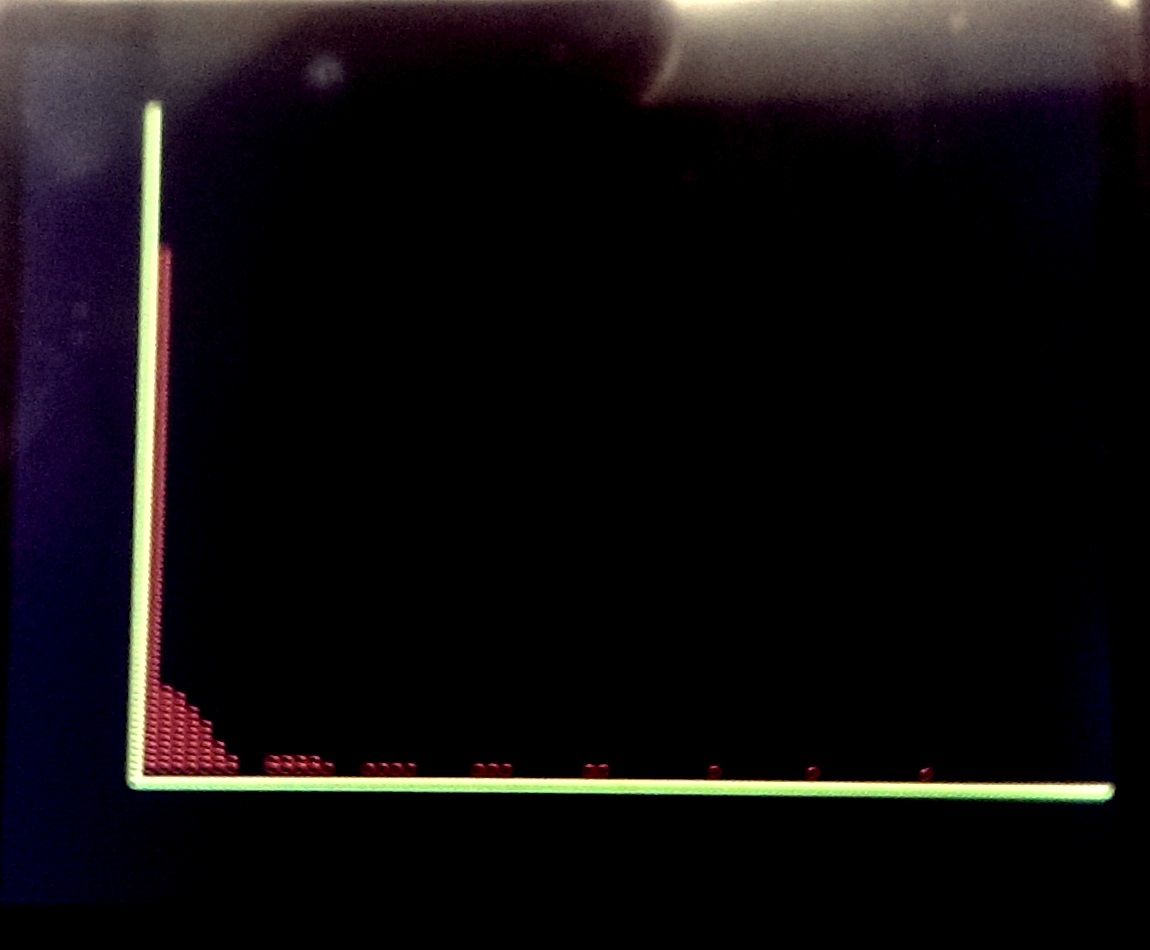
\includegraphics[width=\pica]{Images/P4}
\caption{FFT plot result}
\end{subfigure}
\hspace{5pt}
\begin{subfigure}[H]{\picb}
\center
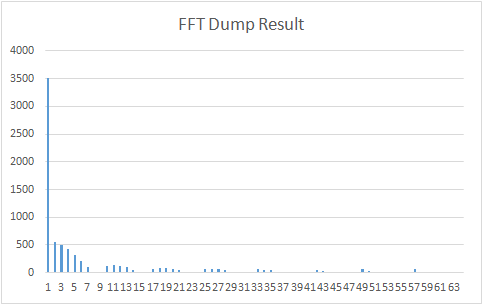
\includegraphics[width=\picb]{Plots/P4}
\caption{FFT dump result}
\end{subfigure}
\caption{FIR filter test data}
\label{fig:Procedure4}
\end{figure}

\section{Analysis and Discussion}

\paragraph{Give the calculations (equations and results) you used to estimate the cutoff frequencies for your HPF and LPF (Preparation 1)? How did the measured frequency response compare to the estimations (procedure 2)?\\}

We wanted the LPF's cutoff to be $400\,Hz$ since we set the sampling rate to $2\,kHz$. Although cutoff is much lower than the maximum allowed
frequency according to Nyquist's theorem, we chose such a low cutoff to be improve performance and prevent aliasing.

Equations:
For a Butterworth 2 Pole Sallen-key LPF, $C_1 = 141.4\,\mu F$ and $C_2 = 70.7\,\mu F$ and $R = 10\,k\Omega$ , $f_c = 1\,Hz$.
To change fc to $400\,Hz$, the new capacitor values can be calculated by $C_1' = \frac{C_1}{2 \pi f_c} = 0.0563\,\mu F$ and
$C_2' = C_1'/2 = 0.0281\,\mu F$. If we multiply the capacitors by $0.344484$ to set $C_1 = 20\,nF$ and $C_2 = 10\,nF$, to keep $f_c$
the same as $400\,Hz$, we should also divide the resistance by $0.344484$ that results in $R = 28.131 k\Omega$.
Finally, we chose the resistance as $27\,k\Omega$ which resulted in a $f_c$ of $416.75\,Hz$.

After doing procedure do we find the cutoff frequency to be around $410\,Hz$. (frequency at which gain was 0.707) This difference is probably due to inaccuracy of resistance and capacitance of the filter components.
 
\paragraph{Explain how you measured maximum bandwidth (procedure 5). What was the limiting factor affecting 
bandwidth?\\}

We added a variable that starts by 0 and is incremented everytime ADC fails to put the sampled data into the FIFO. We also added a separated variable that starts by 0 and is incremented everytime Producer fails has to disregard an old data that is still not displayed by the Display thread. Both variables should be 0 through the test. We started by a low Sampling rate by $2000\,Hz$ and continuously increased it, and read both DataLost variables with or without FIR filter being on. As soon as there was a DataLost in either variable, the bandwidth was determined as the previous step with no DataLost.

Regardless of FIR filter being on or off, liming factor was the display thread as only that variable was incremented as soon as we chose a sampling rate more than the bandwidth. We were able to increase bandwidth by optimizing display functions. (But the system was still limited by the display thread)

We also tested the system with display off and the bandwidth was much higher than before.
 
\paragraph{What is the expected FFT output if the input is a squarewave?\\}
 
Squarewave is the sum of sinewaves with frequencies of $(2n+1)f$ for all $n = 0,1,2,3,\cdots$ where $f$ is the primary frequency of squarewave.

Therefore, the FFT result in the frequency domain should be a impulse train of harmonious frequencies with decreasing strength.
 
\paragraph{Look at the noise in your digital samples when it is very quiet? What type of noise is it? \\}

The noise when we don't move the distance sensor is sudden spikes at random times. (we used distance sensor, not microphone)
 
 \paragraph{We made a big fuss over jitter in labs 2 and 3. Can you estimate the jitter in your ADC samples? \\}
 
 Jitter is 0, since we are using a timer to trigger ADC capture.
 
\paragraph{Prove your FIR implementation can not overflow. \\}

 largest coefficient of the FIR filter $ = 8578 < 2^14$ \\
 The number of points $ = 51 < 2^6 $ \\
 Maximum number of ADC result $ = 4095 < 2^12 $ \\
 
 Maximum total size $ < 2^6 \cdot 2^14 \cdot 2^12 = 2 ^ 32 $ \\
 Therefore, the sum fits in a 32-bit unsigned long variable \\
 
\paragraph{Look at the symmetry in the $h[51]$ coefficients in the example FIR design. How could you rewrite the 
following filter equation to reduce the number of multiplies from 51 to 26? \\}

We could rewrite the filter equation to simplify the calculation as follows
{ \lstset{language=C, frame=none, numbers=none}
\begin{lstlisting}
y[i]= (h[0]*x[i]+h[1]*x[i-1]+h[2]*x[i-2]+...+h[50]*x[i-50])/256;
    = (h[0]*(x[i]+x[i-50]) + h[1]*(x[i-1]+x[i-49] + ... h[25]*(x[i-24]+x[i-26]) + h[26]*x[i-26] ) / 256;
\end{lstlisting}
}

\paragraph{If your system executed the FIR filter using the multiply and accumulate instruction (MLA), you can skip 
this question. Explain how the MLA instruction could have made your filter execute faster? If you were to have 
used the MLA instruction, would it have been more accurate? \\}

The compiler used MLA in the filter implementation,.

MLA is faster than using consecutive MUL and ADD instruction. So, it can potentially speed up the FIlter execution time by a factor of 2. However, since we have a for loop in the system, the effect of the otther instructions cannot be neglected, so execution time will practically increase, but not increase by a factor of 2.


\end{document}